\documentclass[conference]{IEEEtran}

\hyphenation{op-tical net-works semi-conduc-tor}

\usepackage{graphicx}

\makeatletter
\renewcommand{\fnum@figure}{Figure \thefigure}
\makeatother

\begin{document}

\title{A Comparison of DeepMedic and U-Net Neural Network Architectures for Lung Segmentation from Computed Tomography Scans}

\author{
	\IEEEauthorblockN{Daniel Allen}
	\IEEEauthorblockA{
		University of Western Ontario\\
		Email: dallen44@uwo.ca}
	\and
	\IEEEauthorblockN{Rajat Balhotra}
	\IEEEauthorblockA{
		University of Western Ontario\\
		Email: rbalhotr@uwo.ca}
	\and
	\IEEEauthorblockN{Steffen Bleher}
	\IEEEauthorblockA{University of Western Ontario\\
		Email: sbleher@uwo.ca}
	\and
	\IEEEauthorblockN{Lionel Rajaona}
	\IEEEauthorblockA{
		University of Western Ontario\\
		Email: lrajaona@uwo.ca}
}


\maketitle

\begin{abstract}
In this report two deep convolutional neural network architectures for medical image segmentation; DeepMedic and U-Net were compared for performance in the task of automatically creating segmentations of lung structures in clinical computed tomography (CT) scans. The algorithms were trained on a portion of the LUNA16 dataset and the results were compared and evaluated using different metrics for determining segmentation accuracy and quality.
\end{abstract}

\section{Introduction}

% !TEX root = ../Report.tex

Since hardware specifications and computational power increased dramatically in the last years machine learning approaches can be applied in various disciplines today. On top of that the progress in research on convolutional neuronal networks (CNN) made it a very powerful tool for image processing where information is gained from image data.\newline
One challenging application is medical image computing (MIC). The main goal of MIC is to extract clinically relevant information or knowledge from medical images. Furthermore Segmentation is the process of partitioning an image into different meaningful segments (e. g. organs, bones, ...).\newline
In this project the goal is to segment the lung of a human body from computed tomography (CT) scans.\newline
The used dataset is from the LUNA16 challenge \cite{luna} and each scan contains a number of slices which are 512 x 512 pixel greyscale images. The algorithm creates a 512 x 512 pixel label map for each slice marking every pixel that is part of the lung. An example of one scan and the corresponding labeling is shown in figure \ref{scan_picture}.

\begin{figure}[h!]
	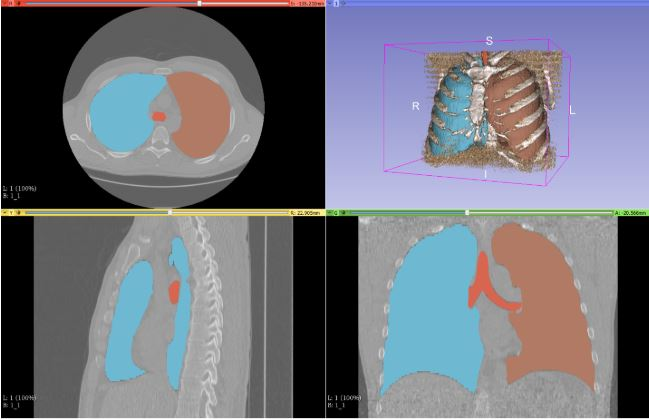
\includegraphics[width=0.49\textwidth, angle=0]{files/scan_picture.jpg}
	\caption{CT scan of the lung and labeled parts}
	\label{scan_picture}
\end{figure}

The segmentation of the lung from the rest of the picture is the first step for further image processing. In the LUNA16 dataset the final goal for example is to detect nodules of the lung indicating cancer. Machine learning approaches can be a powerful support for the doctors who treat patients with suspected cancer. The algorithms can reduce human errors, and it might even have the potential to outperform human capabilities or could automatize the process of cancer detection. This could have a positive effect on health care quality and costs.\newline
In this work two different neuronal networks will be trained and tested to segment the lung on the above described dataset. Furthermore they will be examined and compared under different metrics.\newline
First a short overview on the DeepMedic Network and the U-Net will be given and will be related to other approaches for medical image segmentation. After that the process and implementation will be explained and then the results of the two algorithms will be examined and compared.


\section{Background}
% !TEX root = ../Report.tex
\subsection{DeepMedic architecture}
DeepMedic is a 3D neural network. It has been initially used for segmentations in biomedical 3D scans, especially for detecting brain anomalies such as injuries, tumors and lesions. In this project we will try this algorithm for lung segmentations. \newline
\begin{figure}[h!]
	\includegraphics[width=0.49\textwidth, angle=0]{files/deepmedic.png}
	\caption{Structure of DeepMedic architecture}
	\label{deepmedic}
\end{figure}
 
A DeepMedic model consists of detecting a particular pattern in an image. This is achieved by multi-layer convolution in the network. We distinguish two components in the model. First there is a three-dimension convolutional neural network (CNN) model used for dense segmentation (figure \ref{deepmedic} left part), then  a three-dimension fully connected conditional random field (CRF) model which does post-processing and handles the hard segmentation as well (figure \ref{deepmedic} right part). We can also notice a double-path network composed of a regular-resolution and a lower-resolution path. This second one mainly prevents from overfitting.
Each layer of the CNN model contains channels called feature maps, i.e. a group of neurons identifying a feature in the previous layer. Then featurer are defined by associated kernel weights. Number of inputs, outputs, feature-maps and kernels are tunable.

\subsection{U-Net architecture}
Semantic segmentation is partition of an image in coherent parts. U-Net is mostly used for biomedical image segmentation. In figure \ref{unetstructure} the structure of the U-Net is shown.\newline
\begin{figure}[h!]
	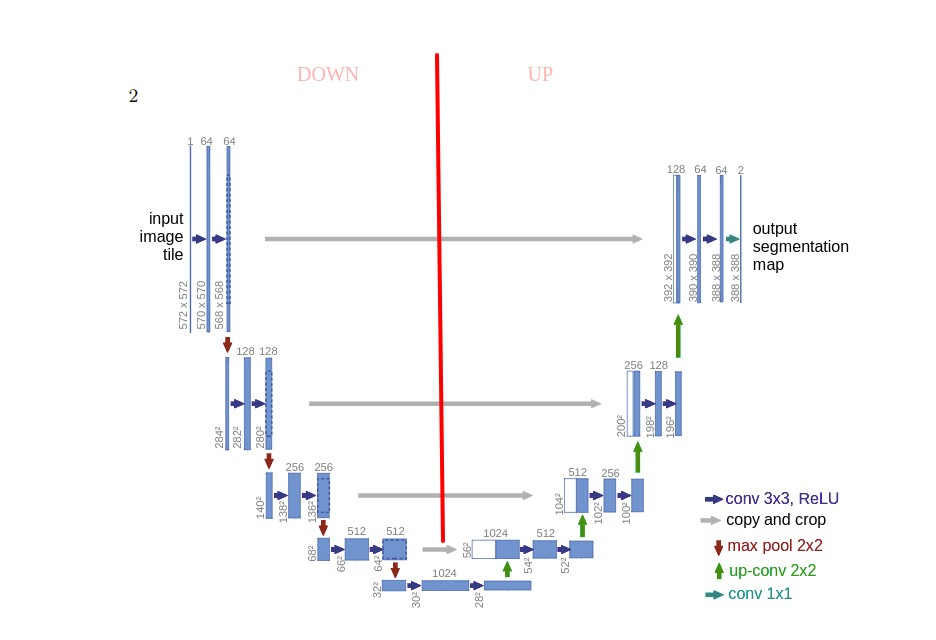
\includegraphics[width=0.49\textwidth, angle=0]{files/unetstructure.jpg}
	\caption{Structure of U-Net architecture}
	\label{unetstructure}
\end{figure}

Each blue box corresponds to a multi-channel feature map. The number of channels is denoted on top of the box. X-Y-size is provided at the lower left edge. White boxes represent copied feature maps. Arrows denote the different operations.\newline
First part is called down or encoder part. Convolutional blocks followed by maxpool downsampling layers are applied to encode the input image into feature representations at multiple different levels. The second part of the network consists of upsampling and concatenation layers followed by regular convolution operations. The dimensions from left are expanded to meet the original image size. The grey and green arrows indicate where to concatenate future maps together.\newline
In comparison to other fully convolutional segmentation networks, the main feature of U-Net  is that while upsampling and going deeper in the networks, it also concatenates the higher resolution features from the down sampling part with upsampled features in order to better localize and learn representation.\newline
%As upsampling is sparse we need to be good prior from beginning stages to get the better localization representation. In order to get consistent size, we applied padded convolutions to keep dimensions across concatenation. Localization is one of the most important features in case of biomedical image processing. In order to localize, high resolution from the contracting path are combined with upsampled output. By this the successive convolution layer can then learn to assemble a more precise output. The main modification in our architecture was that in the upsampling part we have a large number of feature channels, which allows the network to propogate context information to high resolution layers. To predict the pixels in the border region of the image, the missing context is extrapolated by mirroring the input image.

\subsection{Metrics}\label{metrics_chapter}

\subsubsection{Dice Loss}
We need  validation criteria to build our models. We use a Dice loss coefficient to compare the similarity of two samples. In the following equation, smooth is added and stands for backpropagation. Ours is defined by: 
\begin{equation}
dice loss = 1 - \frac{2*(Y_{true} \bigcap Y_{prediction}) + 1}{|Y_{true}| + |Y_{prediction}| + 1}
\end{equation} 



\subsubsection{BCE Dice Loss}
We also use binary cross-entropy (BCE) to measure the performance of our classification model. For labels y and predcted probabilities p, binary cros-entropy is:

\begin{equation}
BCE = - \frac{1}{n} \sum_{i=1}^{n}(y_i \log{(p_i)} + (1-y_i)\log{(1-p_i)})
\end{equation} 


Then, our BCE Dice Loss is:

\begin{equation}
Loss =  dice loss + BCE
\end{equation}

\subsubsection{Hausdorff distance}
The Hausdorff distance is a metric to calculate the maximum of the difference between two sets of coordinates.\newline
For the set of coordinates $A$ and $B$ it is defined as following

\begin{equation}
	d_{hausdorff} (A,B) = \max_{a \in A} (\min_{b \in B} d(a,b))
\end{equation} 

where $d(a,b)$ represents the Euclid distance between the two coordinates $a$ and $b$. It can be interpreted as the maximum distance of set $B$ to set $A$ and is therefore a important metric for evaluating the difference between two label maps.

\subsubsection{Mean distance}
The mean distance is similar to the Hausdorff metric but is a measurement for the mean of the difference between two sets of coordinates.\newline
It is therefore defined as following

\begin{equation}
	d_{mean} (A,B) = \frac{1}{|A|} \sum_{a \in A} \min_{b \in B} d(a,b)
\end{equation}

where again $d(a,b)$ represents the Euclid distance between the two coordinates $a$ and $b$. It furthermore can be seen as the average difference between the two sets and will also be used for evaluation.


\section{Related Work}
% !TEX root = ../Report.tex

Semantic segmentation of anatomical structures from medical image volumes is a common subject of research in biomedical engineering. Traditional techniques pre-dating deeplearning for medical image segmentation include thresholding, atlas-based segmentation, and statistical shape modeling. A paper comparing the capabilities of thresholding, region-based, shape-based, anatomy-guided, and machine learning approaches for segmenting structures in the lungs has been done in 2015 \cite{comparison:article_typical}. This report found that

\section{Methods}
% !TEX root = ../Report.tex

In this section an detailed description of the dataset will be given. The methods of data preprocessing, configuration and training of the two architectures, and predictions for the two architectures will be explained.

\subsection{LUNA16 dataset}

The dataset used in this project was from the LUNA16 challenge consisting of clinical CT scans and corresponding label map segmentations. The goal of the algorithms is to automatically create a label map for each 3D image volume marking every voxel (3D pixel) that is part of the lung or the bronchus with an appropriate label value. An example of one scan and the corresponding segmentation label map is shown in figure \ref{scan_picture}.

\begin{figure}[h!]
	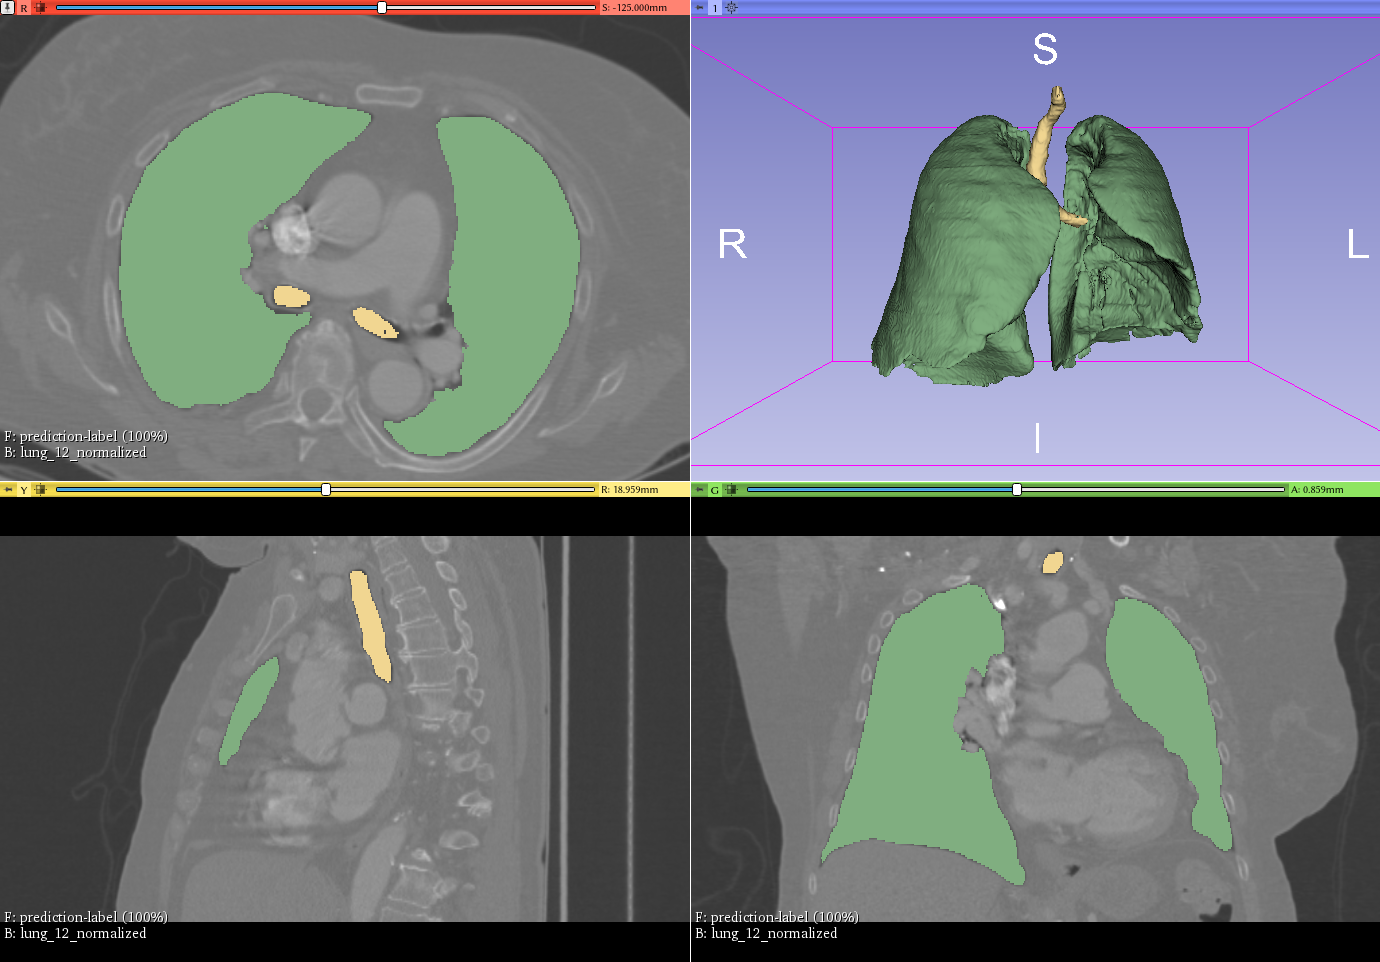
\includegraphics[width=0.49\textwidth, angle=0]{files/Fulllayoutprediction.png}
	\caption{CT scan of the chest with corresponding label map segmentation delineating the lungs (green) and the bronchus (yellow). The first three image portions counterclockwise are the axial, sagittal, and coronal slice views and the final portion is a 3D model of the label.}
	\label{scan_picture}
\end{figure}

The dataset consists of about 10GB of mhd and raw image files. The files contain a varying number of axial slices of 512 x 512 pixel grey-scale images and corresponding 512 x 512 pixel label maps. Since computational resources were limited a subset of the data was used for this work, more specifically 10 CT image volumes for training and 20 CT image volumes for evaluation were chosen randomly from the set. Furthermore the two label categories for the left and right lungs of the LUNA16 dataset was reduced to one label for the lungs and one label for the bronchus since the two chosen image segmentation CNN architectures were not suitable for representing relative positional information.\newline

\subsection{Preprocessing of image data}
Each raw file was converted to a NIfTI format image file for better processing and visualization. These files each contain a 3D greyscale image volume of a chest CT scan. For more appropriate input values, each image volume was normalized separately following the standard normal distribution ($\mu = 0.0$ and $\sigma = 1.0$).\newline
Then, it was necessary to implement data importation to properly use them. Data from directory was converted into input and label matrices following the size $512$ x $512$ x $n$ with the number of all slices in the dataset $n$.

\subsection{Training and validation}
Both network architectures were trained on the 2145 slices of the 10 training CT scans over 35 epochs.\newline
For the DeepMedic architecture a open-source implementation \cite{deepmedic} was modified for the purpose of lung segmentation. RMS propagation with a initial learning rate of 0.001 and Nesterov momentum (momentum value of 0.6), and L1 and L2 regularization (0.000001 and 0.0001 respectively) were used. Furthermore, the learning rate was reduced in later epochs in order to improve convergence. For the training a batch size of 10 samples was chosen from the image volumes and the network was evaluated with the binary cross entropy (BCE) as a loss function.\newline
The U-Net architecture was built according to the structure in figure \ref{unetstructure}. For the training process the Adam optimizer with the described loss function $Loss = dice loss + BCE$ from chapter \ref{metrics_chapter} was used in combination with a batch size of 3 full 512x512 slices. To get an idea of the performance of the model during training and ensure that only well generalized models were being saved 10\% of the 2145 slices were used for validation while the other 90\% were used for training.\newline

\subsection{Managing the large dataset and image volume size}
Although the dataset was reduced to 10 CT scans some adjustment in the training process still had to be made to handle the size of the dataset and individual 3D image volumes.\newline
Therefore, a generator was defined to reduce the data size that will be fed to the training process at once. Thus reducing the VRAM memory load on the GPU. The generator feeds batches of images as required to the training process instead of loading the whole dataset onto the GPU and model fitting process at once.

\subsection{Prediction, displaying and calculating metrics}

After training the two models were used to predict the segmentation label maps of the 20 test CT scans. The predicted labels were again merged to NIfTI files and displayed. For evaluation an average of the dice loss, the Hausdorff distance and the mean distance were calculated over all 20 test scans.

\section{Evaluation}
% !TEX root = ../Report.tex

\subsection{Setup}

Python 3.6 or over can be chosen to design this solution. NiBabel package was used to deal with specificity of medical images. TensorFlow and Keras are additional libraries required to build training models and calculate metrics.

\subsection{Evaluation on training model}
graph loss on training evaluation (dice loss, bce dice loss, batch size (correlates to gpu), epochs, steps per epoch, optimizer)
prediction
image on label and prediction 
evaluating and examining models with hausdorff and mean distance on pictures (graphs or statistics, table)
comparison of unet and deepmedic

explain high hausdorff and how to reduce it


\begin{table}[h!]
	\centering
	\setlength{\tabcolsep}{10pt}
	\renewcommand{\arraystretch}{1.5}
	\begin{tabular}{c c c c}
		\hline 
		Architecture & Dice & Hausdorff & Mean \\
		& Coefficient & distance (mm) & Distance (mm) \\ 
		\hline 
		DeepMedic & 0.968 & 119.50 & 1.45 \\ 
		U-Net & 0.976 & 103.21 & 0.33 \\ 
		\hline
		\newline 
	\end{tabular}
	\caption{Dice Loss, Hausdorff distance and mean distance on 20 evaluation CT scans for the DeepMedic and the U-Net architecture.}
	\label{table_result}
\end{table}

\begin{figure}[h!]
	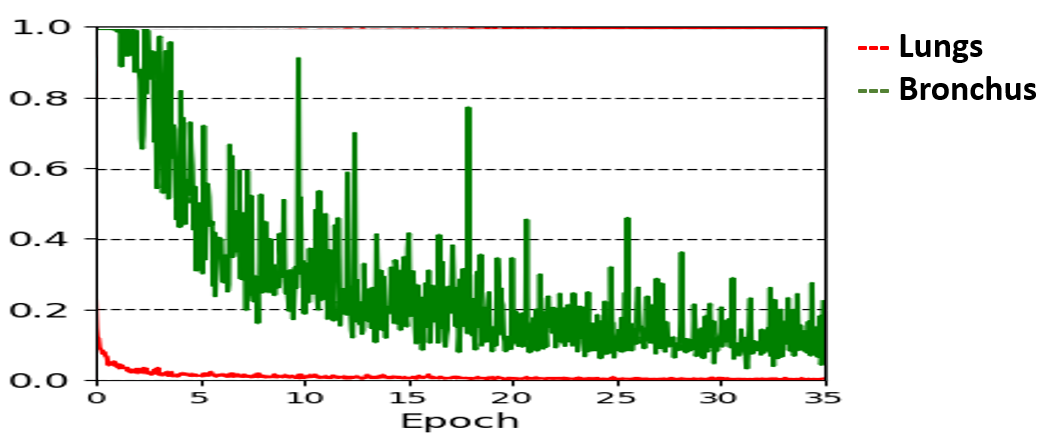
\includegraphics[width=0.49\textwidth, angle=0]{files/deepmedictrain.png}
	\caption{Training process of the DeepMedic architecture. The loss function (BCE) on the training data is shown for the lungs (red) and for the bronchus (green)}
	\label{train_deepmedic}
\end{figure}


\begin{figure}[h!]
	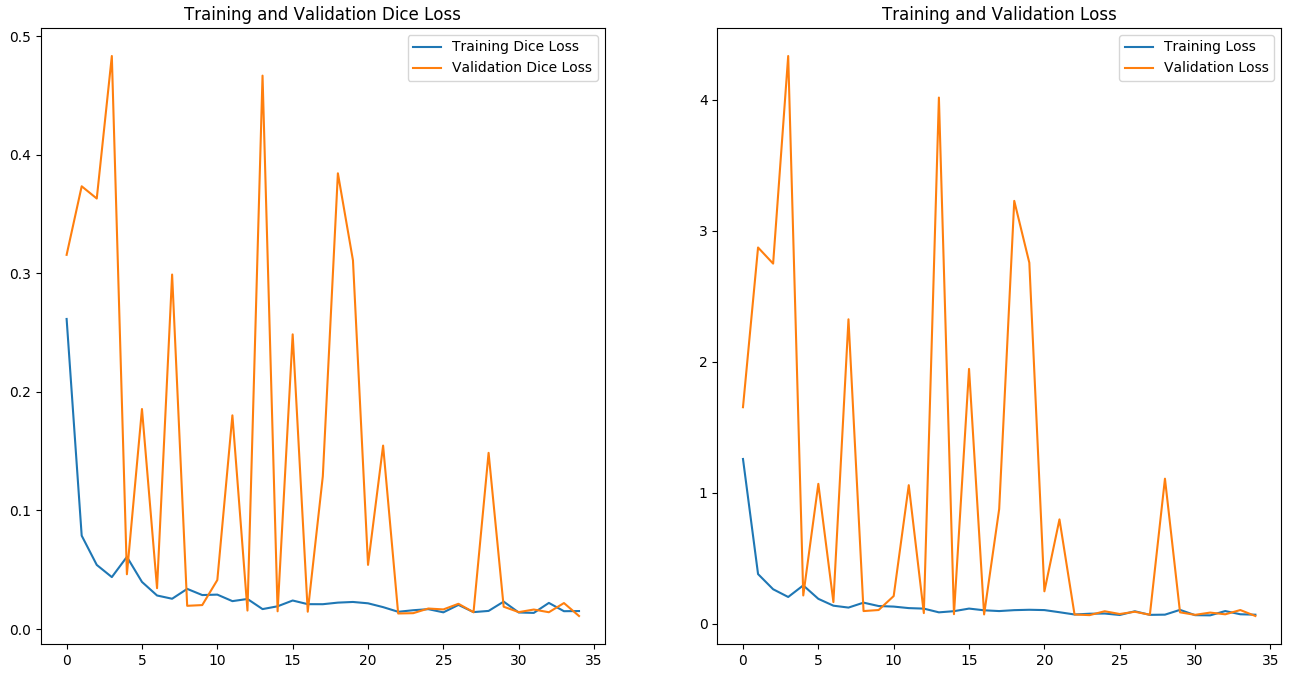
\includegraphics[width=0.49\textwidth, angle=0]{files/jpgunettrain.png}
	\caption{Training process of the U-Net architecture. The dice loss on the training and validation data is shown on the left. The actual loss function ($BCE + dice loss$) is shown on the right.}
	\label{train_unet}
\end{figure}

\begin{figure}[h!]
	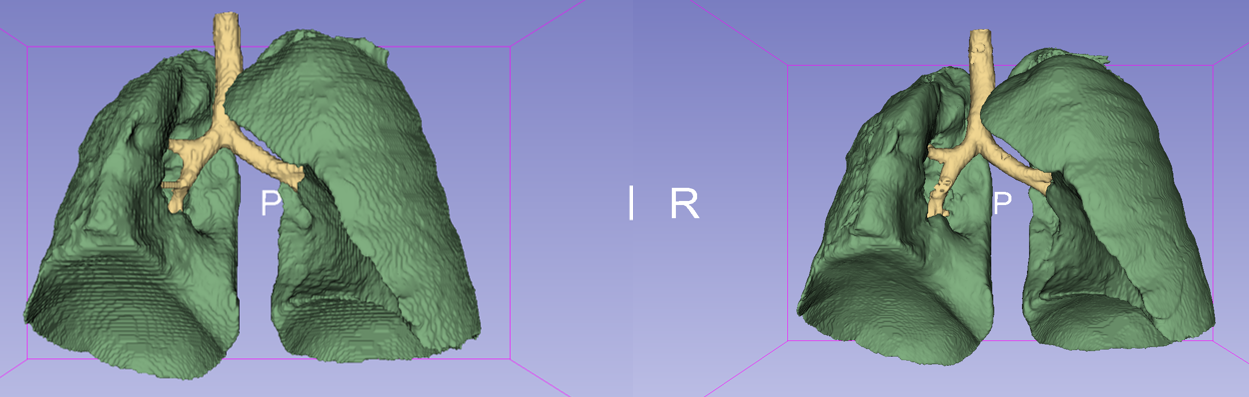
\includegraphics[width=0.49\textwidth, angle=0]{files/preddeepmedic.png}
	\caption{Example prediction of the DeepMedic architecture on one CT scan. The original label map for training is displayed on the left while the prediction of the network is shown on the right.}
	\label{pred_deepmedic}
\end{figure}

\begin{figure}[h!]
	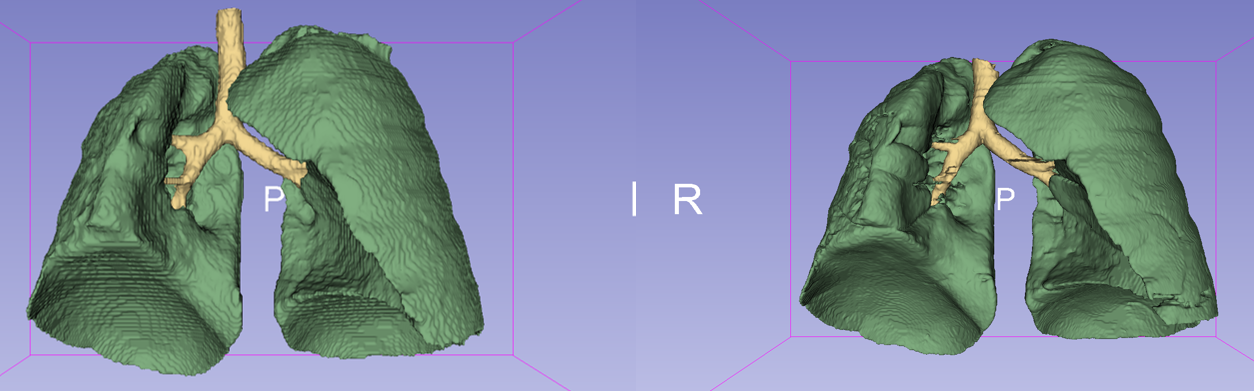
\includegraphics[width=0.49\textwidth, angle=0]{files/predunet.png}
	\caption{Example prediction of the DeepMedic architecture on one CT scan. The original label map for training is displayed on the left while the prediction of the network is shown on the right.}
	\label{pred_unet}
\end{figure}


\section{Summary and conclusion}
% !TEX root = ../Report.tex

In this project different approaches for lung segmentation were examined. The goal was to create a 3D segmentation of the lung from a CT image volume scan consisting of slices. The two deep convolutional neuronal network architectures DeepMedic and U-Net were configured and implemented to be trained on a set of clinical chest CT scans. The predictions of both models were evaluated using the Dice coefficient, the Hausdorff distance and the mean distance as metrics. Both models performed very well on the lung segmentation and created an accurate structure of the lungs and the bronchus. However, the largest difference between the two networks was the consistency of the segmentation of the more difficult to delineate bronchus which the DeepMedic model excelled at, however the training time for DeepMedic was a few hours longer.\newline
To put the work into a larger context it can be said that many differing architectures exist for the difficult and broad task of image segmentation in medical applications. One of the biggest challenges in image segmentation is getting appropriate and reliable data and preparing and augmenting this data for effective model generation for machine learning. On top of that, handling of the exceptionally large datasets and image volumes, reduction of training time and the allocation of computational resources make the task even more challenging and many approaches to these problems need to be assessed for each unique application.\newline
It can be concluded that machine learning today can create valuable new results in medical image processing. In the specific task of lung segmentation the next step after extracting the lung from the CT scans would be to mark cancerous nodules in the lung for cancer detection and treatment. This work is therefore a helpful first step to reach the goal of improved medical treatment through machine learning approaches.

\bibliographystyle{IEEEtran}
\bibliography{bibi}

\end{document}


